\documentclass[12pt]{article}
\usepackage{amssymb}
\usepackage{geometry}
\usepackage{graphicx}
\usepackage[colorlinks=true, allcolors=blue]{hyperref}
\usepackage{cite}
\usepackage{wrapfig}
\usepackage{booktabs}
\usepackage{soul}
\usepackage[most]{tcolorbox}
\usepackage{amsmath}
\usepackage{lipsum}
\usepackage{caption}
\usepackage{ulem}
\usepackage{xcolor}
\usepackage{tikz}
\usetikzlibrary{arrows.meta, positioning, shapes}
\usepackage{sectsty}

%--------- Define Colors ---------
\definecolor{titleColor}{HTML}{800000}        % Maroon
\definecolor{sectionColor}{HTML}{4682B4}      % SteelBlue
\definecolor{subsectionColor}{HTML}{6A5ACD}   % SlateBlue
\definecolor{textHighlight}{HTML}{DAA520}     % Goldenrod
\definecolor{backgroundColor}{HTML}{F0F8FF}   % AliceBlue
\definecolor{emphasisColor}{RGB}{200, 50, 50} % ForestGreen

\sectionfont{\color{sectionColor}}       % Color for \section
\subsectionfont{\color{subsectionColor}} % Color for \subsection

%--------- Custom Highlight Commands ---------
\definecolor{lightblue}{RGB}{230, 240, 255}
\definecolor{lightgreen}{RGB}{220, 255, 220}
\definecolor{lightred}{RGB}{255, 230, 230}
\definecolor{lightyellow}{RGB}{255, 255, 200}
\definecolor{darkblue}{RGB}{0, 51, 102}

\newcommand{\bluehighlight}[1]{\colorbox{lightblue}{#1}}
\newcommand{\greenhighlight}[1]{\colorbox{lightgreen}{#1}}
\newcommand{\redhighlight}[1]{\colorbox{lightred}{#1}}
\newcommand{\yellowhighlight}[1]{\colorbox{lightyellow}{#1}}
\newcommand{\blue}[1]{\textcolor{darkblue}{#1}}
\newcommand{\myemphasis}[1]{\textcolor{emphasisColor}{\textbf{#1}}}

%--------- Color Blocks ---------
\newtcolorbox{blockA}{
  breakable,
  colback=blue!5,
  colframe=blue!40!black,
  enhanced,
  boxrule=0.7pt,
  arc=2mm,
  left=4mm,right=4mm,top=2mm,bottom=2mm
}

\newtcolorbox{blockB}{
  breakable,
  colback=red!5,
  colframe=red!40!black,
  enhanced,
  boxrule=0.7pt,
  arc=2mm,
  left=4mm,right=4mm,top=2mm,bottom=2mm
}

\newtcolorbox{blockC}{
  breakable,
  colback=green!5,
  colframe=green!40!black,
  enhanced,
  boxrule=0.7pt,
  arc=2mm,
  left=4mm,right=4mm,top=2mm,bottom=2mm
}

\newtcolorbox{blockD}{
  breakable,
  colback=purple!5,
  colframe=purple!40!black,
  enhanced,
  boxrule=0.7pt,
  arc=2mm,
  left=4mm,right=4mm,top=2mm,bottom=2mm
}

%--------- Title ---------
\title{\textcolor{titleColor}{\textbf{\Huge Digital Life: \color{blue} Electronic Commerce:\\ \textit {\large  \color{red} Analytical Innovations }}}}

\author{B. M. Osman\thanks{Al Nahada University, Cairo \\ \texttt{babikerosman@yahoo.com}}}
\date{\today}
\begin{document}
\maketitle

\section{Introduction}

Electronic commerce (e-commerce) has transformed the way businesses interact with customers, suppliers, and partners. The rapid growth of digital platforms has generated vast amounts of transactional and behavioral data. Analytical innovations enable organizations to extract meaningful insights from these data, leading to improved operational efficiency, enhanced customer experiences, and better strategic decision-making.

\section{Key Analytical Innovations in Electronic Commerce}

\begin{enumerate}

\item \textbf{Artificial Intelligence (AI)}
\begin{itemize}
    \item Personalized product recommendations.
    \item Intelligent chatbots and virtual assistants.
    \item Automated customer service.
    \item Demand forecasting.
\end{itemize}

\item \textbf{Machine Learning (ML)}
\begin{itemize}
    \item Customer behavior prediction.
    \item Fraud detection.
    \item Dynamic pricing.
    \item Recommendation engines.
\end{itemize}

\item \textbf{Big Data Analytics}
\begin{itemize}
    \item Processing massive customer datasets.
    \item Sales trend analysis.
    \item Marketing performance evaluation.
    \item Supply chain optimization.
\end{itemize}

\item \textbf{Predictive Analytics}
\begin{itemize}
    \item Sales forecasting.
    \item Inventory optimization.
    \item Customer lifetime value estimation.
    \item Churn prediction.
\end{itemize}

\item \textbf{Customer Segmentation}
\begin{itemize}
    \item Behavioral segmentation.
    \item Demographic analysis.
    \item Personalized marketing campaigns.
    \item Customer profiling.
\end{itemize}

\item \textbf{Sentiment Analysis}
\begin{itemize}
    \item Review mining.
    \item Social media monitoring.
    \item Brand reputation analysis.
    \item Customer satisfaction assessment.
\end{itemize}

\item \textbf{Real-Time Analytics}
\begin{itemize}
    \item Live website monitoring.
    \item Instant transaction analysis.
    \item Real-time fraud alerts.
    \item Immediate inventory updates.
\end{itemize}

\item \textbf{A/B Testing}
\begin{itemize}
    \item Website optimization.
    \item Marketing campaign evaluation.
    \item User interface improvements.
    \item Conversion rate optimization.
\end{itemize}

\item \textbf{Network and Graph Analytics}
\begin{itemize}
    \item Customer relationship analysis.
    \item Product association mining.
    \item Supply network optimization.
    \item Recommendation enhancement.
\end{itemize}

\item \textbf{Blockchain Analytics}
\begin{itemize}
    \item Secure payment verification.
    \item Supply chain traceability.
    \item Transaction transparency.
    \item Digital identity management.
\end{itemize}

\end{enumerate}

\section{Business Benefits}

Analytical innovations provide numerous advantages:

\begin{itemize}
    \item Increased sales and revenue.
    \item Enhanced customer satisfaction.
    \item Improved operational efficiency.
    \item Better inventory management.
    \item Reduced fraud and financial risk.
    \item Data-driven strategic planning.
    \item Personalized customer experiences.
    \item Competitive advantage in digital markets.
\end{itemize}

\section{Future Trends}

Emerging technologies are expected to further transform electronic commerce analytics:

\begin{itemize}
    \item Generative Artificial Intelligence.
    \item Explainable AI (XAI).
    \item Autonomous commerce systems.
    \item Edge analytics.
    \item Quantum computing for optimization.
    \item Digital twins of supply chains.
    \item Federated learning for privacy-preserving analytics.
    \item Sustainable and green e-commerce analytics.
\end{itemize}


\section{Available Resources}

\begin{itemize}
    \item \textbf{HP All-in-One PC (64-bit)} -- Central Server
    \item \textbf{HP OmniBook X Laptop (17.3")} -- Development and Analytics Workstation
    \item \textbf{Android Smartphone with Termux and Debian} -- Mobile Administration and Data Collection
\end{itemize}

\begin{figure}[htbp]
\centering

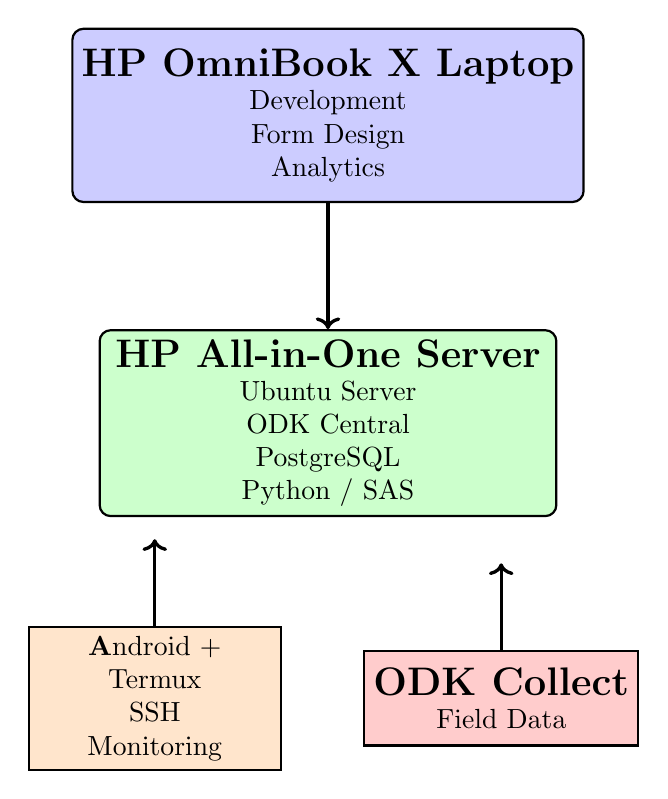
\begin{tikzpicture}[
node distance=1.6cm,
box/.style={
rectangle,
rounded corners,
draw,
thick,
minimum width=5.8cm,
minimum height=2.2cm,
align=center
},
smallbox/.style={
rectangle,
draw,
thick,
minimum width=3.2cm,
minimum height=1.2cm,
align=center
},
arrow/.style={->,very thick}
]

% Laptop
\node[box,fill=blue!20] (laptop)
{\Large\textbf{HP OmniBook X Laptop}\\
Development\\
Form Design\\
Analytics};

% Server
\node[box,fill=green!20,below=of laptop] (server)
{\Large\textbf{HP All-in-One Server}\\
Ubuntu Server\\
ODK Central\\
PostgreSQL\\
Python / SAS};

% Bottom boxes
\node[smallbox,fill=orange!20] (termux)
at ([xshift=-2.2cm,yshift=-2.3cm]server.south)
{\textbf Android + \\Termux\\
SSH\\
Monitoring};

\node[smallbox,fill=red!20] (collect)
at ([xshift=2.2cm,yshift=-2.3cm]server.south)
{\Large\textbf{ODK Collect}\\
Field Data};

% Arrows
\draw[arrow] (laptop) -- (server);
\draw[arrow] (termux.north) -- ++(0,1.1cm);
\draw[arrow] (collect.north) -- ++(0,1.1cm);

\end{tikzpicture}

\caption{Digital Health Infrastructure Architecture}
\end{figure}


\begin{figure}[htbp]
\centering

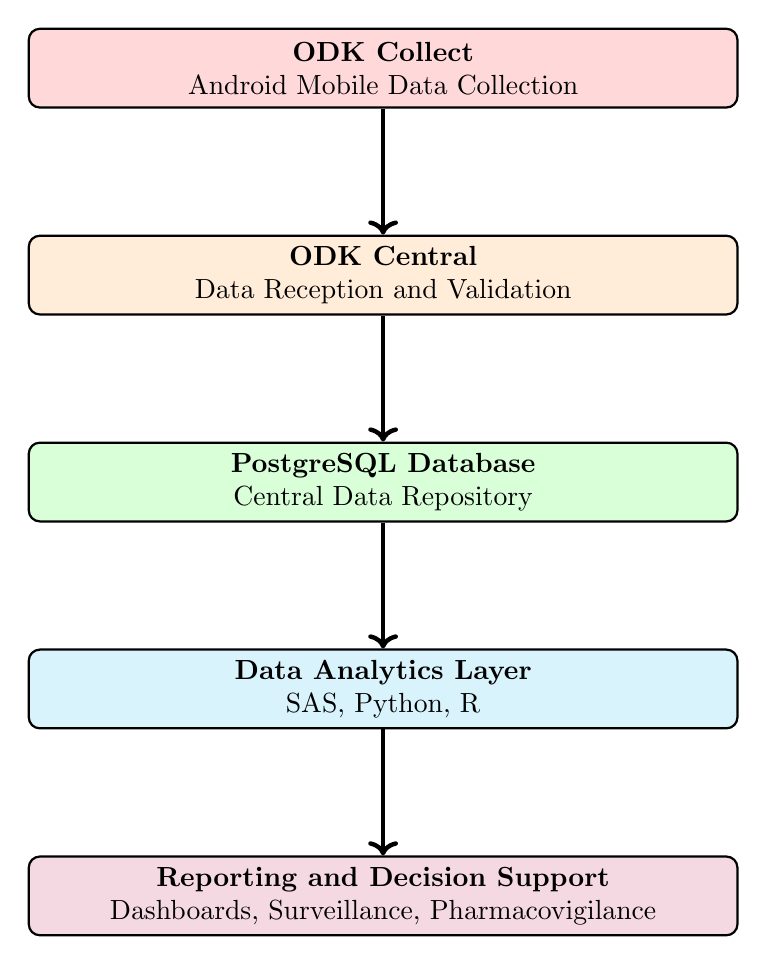
\begin{tikzpicture}[
node distance=1.6cm,
box/.style={
rectangle,
rounded corners,
draw,
thick,
minimum width=9cm,
minimum height=1cm,
align=center
},
arrow/.style={
->,
ultra thick
}
]

\node[box, fill=red!15] (a)
{\textbf{ODK Collect}\\
Android Mobile Data Collection};

\node[box, fill=orange!15, below=of a] (b)
{\textbf{ODK Central}\\
Data Reception and Validation};

\node[box, fill=green!15, below=of b] (c)
{\textbf{PostgreSQL Database}\\
Central Data Repository};

\node[box, fill=cyan!15, below=of c] (d)
{\textbf{Data Analytics Layer}\\
SAS, Python, R};

\node[box, fill=purple!15, below=of d] (e)
{\textbf{Reporting and Decision Support}\\
Dashboards, Surveillance, Pharmacovigilance};

\draw[arrow] (a) -- (b);
\draw[arrow] (b) -- (c);
\draw[arrow] (c) -- (d);
\draw[arrow] (d) -- (e);

\end{tikzpicture}

\caption{ODK-Based Data Collection and Analytics Workflow}
\end{figure}


\begin{center}
\begin{tabular}{|p{4cm}|p{8cm}|}
\hline
\rowcolor{blue!15}
\textbf{Component} & \textbf{Primary Role} \\
\hline

HP All-in-One PC &
ODK Central Server, PostgreSQL Database, Analytics Engine
\\
\hline

HP OmniBook X &
Form Design, Training, Data Analysis, Research
\\
\hline

Android + Termux &
Remote Administration, SSH Access, Monitoring
\\
\hline

ODK Collect &
Field Surveys, Public Health Surveillance, Data Capture
\\
\hline

\end{tabular}
\end{center}

\subsection{Applications}

This infrastructure provides a low-cost, scalable platform suitable for other areas of research such as:

\begin{itemize}
    \item Infectious Disease Modelling
    \item Pharmacovigilance
    \item Digital Health Training
    \item Epidemiological Surveillance
    \item Humanitarian Data Collection
    \item Public Health Research
    \item Monitoring and Evaluation Programs
\end{itemize}
\section{Conclusion}

Analytical innovations have become a cornerstone of modern electronic commerce. By integrating artificial intelligence, machine learning, big data analytics, predictive modeling, blockchain technologies, and real-time decision support, organizations can optimize business processes, improve customer engagement, and maintain sustainable competitive advantages in an increasingly digital marketplace.

\end{document} 


